% !TEX root = deckblatt2b.tex

\section{Integrierer}

\begin{figure}[H]
 \centering
 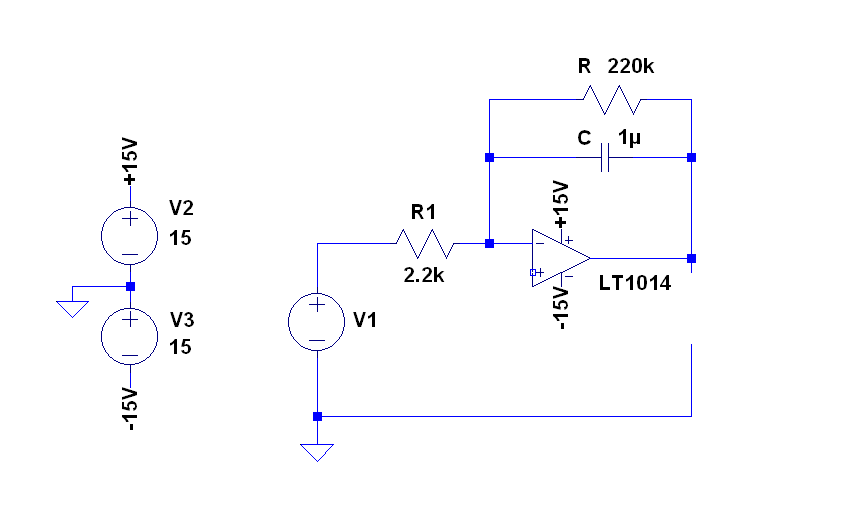
\includegraphics[height=8cm,width=12cm]{Simulationen/Integrator}
 \caption{Operationsverstärker als Integrator beschaltet}
\end{figure}
\noindent
In dieser Beschaltung gibt die Ausgangsspannung das Integral der Eingangsspannung über die Zeit an. Der Widerstand $R$ dient nur zur stabilisation
der Schaltung und wird daher vernachlässigt, er sollte jedoch wesentlich größer als $R_1$ gewählt werden.

\subsection{Übertragungsfunktion}

Der invertierende Integrierer ist vom Aufbau ähnlich dem invertierenden Verstärker, jedoch wird die Ausgangsspannung hier durch die Spannung am Kondensator beschrieben.\\
\begin{align*}
 U_C &= \frac{1}{C} \int i_c(t)\ \mathrm{d}t\\
 i_c &= I_{R1}\\
 U_C &= \frac{1}{RC} \int U_e(t)\ \mathrm{d}t\\
 U_a &= -U_C\\
\end{align*}
\noindent
Aus dieser Berechnung ergibt sich für das Eingangssignal, in Form einer Rechteckspannung mit fallender Flanke, eine Dreiecksspannung mit steigender Flanke.\\
\begin{align*}
 RC &= 2,2ms\\
 U_e(t) &= 
  \begin{cases}
   \ -\frac{1}{10}\ &0 \leq t < 100ms\\
   \quad \frac{1}{10}\ &100ms < t \leq 200ms\\ 
  \end{cases}
  \quad
  U_a(t) = 
  \begin{cases}
   \quad \frac{t}{22}\ &0 \leq t < 100ms\\
   \ -\frac{t}{22}\ &100ms < t \leq 200ms\\ 
  \end{cases}
\end{align*}

Dieses Ergebnis kann man, nach dem Einschwingvorgang, auch in der Simulation beobachten.\\

\begin{figure}[H]
  \centering
  \begin{tikzpicture}
    \begin{axis}[width=15cm, height=10cm, xmin=0, xmax=2, xlabel={t}, ylabel={$U_e$},y tick label style={grid=major}]
      \addplot table[x=time, y=V(n003), mark=none] {csv_files/Integrator_Ue.csv};
      \addplot table[x=time, y=V(n002), mark=none] {csv_files/Integrator_Ua.csv};
    \end{axis}
  \end{tikzpicture}
  \caption{$U_e$ symmetrisches Recktecksignal, $V_{PP}=0.2V, f=5Hz$}
\end{figure}

\subsection{Bode-Diagramm}

\begin{figure}[H]
  \centering
  \begin{tikzpicture}
    \begin{axis}[width=15cm, height=7cm, xmin=1, xmax=100e3, , xmode=log, xlabel={$Hz$}, ylabel={dB},y tick label style={grid=major}]
      \addplot table[x=Freq, y=V(n002),col sep=comma, mark=none] {csv_files/Integrator_dB.csv};
      %\addplot table[x=Freq, y=Phi,col sep=comma, mark=none] {csv_files/Integrator_Phi.csv};
    \end{axis}
  \end{tikzpicture}
  \caption{Frequenzgang}
\end{figure}
\begin{figure}[H]
  \centering
  \begin{tikzpicture}
    \begin{axis}[width=15cm, height=7cm, xmin=1, xmax=100e3, , xmode=log, xlabel={$Hz$}, ylabel={dB},y tick label style={grid=major}]
      %\addplot table[x=Freq, y=V(n002),col sep=comma, mark=none] {csv_files/Integrator_dB.csv};
      \addplot table[x=Freq, y=Phi,col sep=comma, mark=none] {csv_files/Integrator_Phi.csv};
    \end{axis}
  \end{tikzpicture}
  \caption{Phasengang}
\end{figure}

Das Bode-Diagramm zeigt die Abnahme der Verstärkung bei steigender Frequenz, mit $20dB/DEK$. Die Transitfrequenz liegt bei dieser OPV-Schaltung
bei ca. $30Hz$, danach wirkt er dämpfend.\\
